\documentclass{article}
\usepackage{nips10submit_e,times}
%\documentstyle[nips07submit_09,times]{article}
\usepackage[square,numbers]{natbib}
\usepackage{amsmath, epsfig}
\usepackage{amsfonts}
\usepackage{subfigure}
\usepackage{graphicx}
\usepackage{amsfonts}
\usepackage{algorithm}
\usepackage{algorithmic}
\usepackage{easybmat}
\usepackage{footmisc}
\usepackage{subfig}
\renewcommand\algorithmiccomment[1]{// \textit{#1}}
%
\newcommand{\ignore}[1]{}
\newcommand{\comment}[1]{}
\DeclareMathOperator*{\argmax}{arg\,max}







\title{\large{Time Dependent Dirichlet Process Mixture Models\\ for Multiple Target Tracking}}


\author{
Willie Neiswanger \hspace{1cm} Frank Wood\\
Columbia University, New York, NY 10027, USA \\
\texttt{wdn2101@columbia.edu, fwood@stat.columbia.edu}
%\texttt{\{stud1@otherdepth.,\{stud3,fwood\}@stat.,\{stud2\}@columbia.edu}
%\texttt{pfau@neurotheory.columbia.edu} 
%\texttt{\{bartlett,fwood\}@stat.columbia.edu} 
}






% The \author macro works with any number of authors. There are two commands
% used to separate the names and addresses of multiple authors: \And and \AND.
% Using \And between authors leaves it to \LaTeX{} to determine where to break
% the lines. Using \AND forces a linebreak at that point. So, if \LaTeX{}
% puts 3 of 4 authors names on the first line, and the last on the second
% line, try using \AND instead of \And before the third author name.
\newcommand{\fix}{\marginpar{FIX}}
\newcommand{\new}{\marginpar{NEW}}
\newcommand{\X}{\mathcal{X}}
\nipsfinalcopy







\begin{document}

\maketitle







\begin{abstract}
This paper proposes a Multiple Target Tracking (MTT) technique intended to reduce the need for explicit target identification and serve as a general method to track targets with arbitrary characteristics moving over diverse backgrounds. The technique makes use of a known time dependent Dirichlet process mixture model, comprised of a sequence of interdependent infinite Gaussian mixture models constructed to accommodate behavior that changes over time. This paper describes how pixel location values can be extracted from a wide variety of videos containing multiple moving targets and clustered using the aforementioned model in order to perform MTT. The technique is demonstrated on video segments showing multiple ant targets, of distinct species and with diverse physical and behavioral characteristics, moving over non-uniform backgrounds.
\end{abstract}







\section{Introduction}
\label{sec:introduction}

Multiple Target Tracking (MTT) is a machine vision problem that involves identifying multiple concurrently moving targets in a video and maintaining identification of these targets over time while tracking the frame-by-frame locations of each. Difficulties in producing a single, general-purpose algorithm capable of successfully carrying out MTT over a wide range of videos are mainly due to the potential for videos to be highly dissimilar; parameters such as the targets' physical characteristics (including size, shape, color, and behavioral patterns), backgrounds over which the targets move, and filming conditions may all differ. This paper describes the use of a time dependent Dirichlet process mixture model to carry out clustering on data that can be extracted in a general manner from videos containing multiple moving targets. This clustering is incorporated into a general MTT technique for use on a large variety of videos.

Most MTT methods expand upon an algorithmic framework consisting of a target identification phase and a data association phase (see \cite{1521260} and \cite{probmethods} for review of methods). The former phase aims to return a position value for each target in each frame of a video, and is usually accomplished by detecting some sort of distinctive target attribute or filming the targets in a structured environment where a homogeneous, computationally discernible background can be chosen that contrasts with the targets. The latter phase is often carried out probabilistically using, for example, probabilistic data association filters that allow potential location-sequences to be evaluated, and then selected or rejected as target paths. Much research has gone into data association filters that aim to help with a chief MTT hindrance, where the target identification phase returns many false positive positions (clutter) or true negative positions (detection holes).

The clustering-based MTT technique of this paper deviates from the usual two-phase method outlined above in that it does not explicitly carry out target identification. This technique was initially developed to aid ant tracking software intended to track ants of many species, having highly variable physical characteristics, filmed in numerous environments. Hence, the MTT methods in this software could not depend upon any characteristic specific to a given ant species or background property, and needed to instead use video features common to moving targets in any video. This technique begins by extracting three-dimensional location values $(x$, $y$, frame number$) \in \mathbb{R}^{2} \times \mathbb{Z}_{+}$ of certain pixels that tend to be present around moving targets. The extracted pixel location values are distributed roughly as worm-like shapes that follow the paths of individual targets when plotted in $\mathbb{R}^{2} \times \mathbb{Z}_{+}$, where we let the frame number (which can be viewed as a discrete representation of time) ascend the vertical axis (see Data section for further details). Clustering can then be performed with a time dependent Dirichlet process mixture model, which allows each worm-like data cloud to be isolated and examined separately. Regression can be carried out on each isolated data cluster to find a sequence of locations for each target, therby completing the MTT process.

In the following sections, the MTT process and its associated model are discussed in more detail; the process is then demonstrated on video segments containing multiple targets with varied characteristics moving concurrently over diverse backgrounds. 







\section{Data Extraction}

Extraction of three dimensional location values $(x$, $y$, frame number$) \in \mathbb{R}^{2} \times \mathbb{Z}_{+}$ of pixels found near moving targets in videos is necessary to produce worm-like data clouds that can be clustered using the time dependent Dirichlet Process mixture model. One specific way of extracting the location values of relevant pixels is simple frame-differencing, which involves looking at the difference in pixel intensity or value in successive frames, and recording the positions of the pixels (or pixel groups) that have exhibited frame-wise change beyond a given threshold. Frame differencing was the main method used to generate the pixel location values in this project (however, note that the techniques described in the following sections can be applied to any pixel filtering technique producing data that, when plotted, form discernible worm-shaped clouds that trace the paths of targets).

Frame differencing is a rudimentary process, which is advantageous here, since it lends itself well to many MTT situations that can be encoutered. We have found that, when correctly implemented, it is sufficiently general to extract the desired worm-like data clouds from a wide variety of videos containing multiple moving targets with only a few restrictions on the filming conditions (relating to video stability) and target characteristics (which are described in detail in the Experiments section). Additionally, frame differencing can be applied to videos of arbitrary targets, and does not involve the identification of specific target characteristics, which is a desirable trait of this MTT technique.







\section{Model Overview}

The generalized Polya urn dependent Dirichlet process mixture model (GPUDPM) \cite{Caron2007}, described by Caron et al. [2007], is the specific time dependent Dirichlet process mixture model applied in this work. In order to introduce this model, we will begin by providing a brief overview of the (non-dependent) Dirichlet Process Mixture Model (DPMM).

A DPMM is formulated by allowing the mixing distribution in a standard mixture model to be distributed according to a Dirichlet Process (DP); this allows for modeling data where the true number of latent mixture components is unknown and arbitrarily large by assuming an infinite number of components, of which only a finite amount are expressed by the data. In particular, the DPMM can be defined as
\begin{align}
\begin{split}
	x_{i}|\theta_{i} &\sim F(\theta_{i}) \\
	\theta_{i} | \mathbb{G}  &\sim  \mathbb{G} \\
	\mathbb{G} | \alpha, \mathbb{G}_{0}  &\sim  DP(\alpha, \mathbb{G}_{0})
\end{split}
\end{align}
where the $x_{i}$ (for $i \in \{ 1, \ldots, N \}$) are observations, the $\theta_{i}$ are parameters defining the mixture component (i.e. the distribution to be mixed, $F(\theta_{i})$) from which the $i_{th}$ observation is drawn, and the $\theta_{i}$ are drawn from $\mathbb{G}$, which is in turn drawn from a DP with base distribution $\mathbb{G}_{0}$ and parameter $\alpha$ (which can be intuitively viewed as the mean and precision of the DP, respectively). See \cite{Gasthaus2008} and \cite{Gasthaus_thesis} for more details on this formulation.

Let $K$ be the number of distinct mixture components in the above model. We can write the distinct mixture components as $\phi_{1}, \ldots, \phi_{K}$. Let $c_{1}, \ldots, c_{N}$ (where $c_{i} \in \{1, \ldots, K \}$) be class assignment variables that indicate the cluster to which observation $x_{i}$ is assigned. The DPMM can be represented by a Chinese Restaurant Process (CRP), a discrete-time stochastic process that defines a partition of the set $\{ x_{1}, \ldots, x_{N} \}$ (via the elements' assignments $c_{1}, \ldots, c_{N}$) at each time-step. The CRP allows samples to be drawn from the conditional distribution of the indictor variables $c_{i}$, and can be expressed as
\begin{align}
\begin{split}
	P(c_{i} = c_{j} $ for some $ j<i) &= \frac{m_{k}}{i-1+\alpha}\\
	P(c_{i} \neq c_{j} $ for all $ j<i) &= \frac{\alpha}{i-1+\alpha}
\end{split}
\end{align}
where $m_{k}$ is the cardinality of the set $\{ c_{j} | (c_{j}=c_{i}=k)  \wedge  (j < i) \}$ and $\alpha$ is the parameter of the DP prior on $\mathbb{G}$ .

Consider the situation where the distribution of the observations is not static, but evolves over time (for example, in cases where the number, location, and density of clusters is time dependent). In this case, a time dependent DPMM (see \cite{griffinsteel} for formal description of dependent DPMMs), such as the GPUDPM can be used to model the data. A GPUDPM that models data over T discrete time steps can be viewed as a collection of DPMMs (one for each $t \in \{1, \ldots, T \}$), which are linked together by dependencies among their respective parameters. For example, mixture component parameters at a given time step are dependent upon the mixture component parameters in adjacent time steps and the distribution and number of distinct cluster assignments at a given time step are dependent upon the same over a wider range of time steps (and upon a deletion procedure, described below).

To link together the parameters of mixture components in adjacent time-steps, a transition kernel $P(\phi_{k}^{t} | \phi_{k}^{t-1})$ is implemented, which provides a distribution over parameters of a mixture component in a given time-step (as a function of equivalent parameters in adjacent time-steps). One caveat is that each mixture component must be drawn independently from $\mathbb{G}_{0}$, which we achieve by making $\mathbb{G}_{0}$ the invariant distribution of $P(\phi_{k}^{t} | \phi_{k}^{t-1})$ (note that the transition kernel is a markov chain). Additionally, to account for varying numbers of clusters, there is a deletion procedure (described in Caron et al. [2007]) by which observations are considered "removed" from their assigned clusters at a given time-step (which modifies the value of $m_{k}$ defined above). We introduce variables $d_{1}, \ldots, d_{N}$ which denote the times at which the assignments of given observations are considered to be removed. With these variables, we can now express the $m_{k}$ value at time $t$ as
\begin{equation}
m_{k,t} = \sum_{t' = 1}^{t} \mathbb{I}[(c_{t'}=k) \wedge (t < d_{t'})]
\end{equation}
where $\mathbb{I}[\cdot]$ is an indicator function that evaluates to 1 if its argument is true, and 0 otherwise. Additionally, for an observation $x_{i}$ at a given time-step $t$, the deletion time $d_{i}$ can be defined to be $d_{i} = t + l_{i}$, where $l_{i}$ is considered the lifespan of an assignment, is distributed geometrically, and can be expressed as
\begin{equation}
l_{i} | \rho  \sim  \rho(1 - \rho)^{l_{i}}
\end{equation} \\
with parameter $\rho$. This process adheres to what Caron et al. [2007] consider a uniform deletion strategy over all the observations' assignments (since assignments to each cluster have equal probability of being deleted), though a more complex deletion strategy, dependent upon cluster size, can also be implemented.







\section{Model Specification and Inference}

We now specify the particular modeling choices made when implementing the GPUDPM introduced above and describe the inference procedure---which makes use of a Markov Chain Monte Carlo (MCMC) sampler---to sample from the posterior distribution of the model's parameters (closely following the processes described in \cite{Gasthaus2008} and \cite{Gasthaus_thesis}) and perform clustering on the data.

The likelihood function (i.e. the distribution $F(\theta_{i})$ to be mixed in the DPMM) is chosen to be multivariate normal. In particular, the probability of observation $x_{i}$, given the Gaussian component specified by parameters $\phi_{k}$ can be defined to be
\begin{equation}
P(x_{i}|\phi_{k}) := \mathcal{N}(x_{i}|\phi_{k}) = \mathcal{N}(x_{i}|\mathbf{\mu}_{k}, \Lambda_{k}^{-1})
\end{equation}
where the Gaussian component's parameters are $\phi_{k} = \{ \mathbf{\mu}_{k}, \Lambda_{k}^{-1} \}$. However, restrictions will be placed on the covariance matrix $\Lambda_{k}^{-1}$;  in particular, the covariance matrix is restricted to be a diagonal matrix, of the form $\Lambda_{k}^{-1} = \mathbf{\lambda}_{k}\mathbf{I}_{D} = diag(\lambda_{k}^{(1)}, \ldots, \lambda_{k}^{(D)})$, which provides computational advantages when performing inference in the GPUDPM model. This makes the likelihood function a product of univariate normal distributions, one for each of the D dimensions of an observation. We can now reformulate the previous equation as
\begin{equation}
P(x_{i}|\phi_{k}) = \mathcal{N}(x_{i}|\mathbf{\mu}_{k}, \mathbf{\lambda}_{k}\mathbf{I}_{D}) = \prod_{d=1}^{D} \mathcal{N}(x_{i}^{(d)}|\mathbf{\mu}_{k}^{(d)}, \mathbf{\lambda}_{k}^{(d)})
\end{equation}
where terms with the superscript, $(\cdot)^{(d)}$, denote the $d^{th}$ scalar component of a multidimensional form. We now choose the base distribution $\mathbb{G}_{0}$, which serves as a prior for the cluster parameters, to be a product of Normal-Gamma distributions. This form is chosen so that the base distribution is the conjugate prior to the diagonal formulation of the likelihood above. Hence we can define the base distribution to be
\begin{equation}
\mathbb{G}_{0}(\mu_{k}, \lambda_{k} | \mu_{0}, n_{0}, a, b) := \prod_{d=1}^{D}[\mathcal{N}(\mu_{k}^{(d)} | \mu_{0}^{(d)}, n_{0} \lambda_{k}^{(d)})   Ga(\lambda_{k}^{(d)} | a,b)]
\end{equation}
where $\mu_{k}$ and $\lambda_{k}$ are parameters of a Gaussian component (at a given time-step), and $\mu_{0}$, $n_{0}$, $a$, and $b$ are parameters of the base distribution. As previously discussed, the transition kernel $P(\phi_{k}^{t} | \phi_{k}^{t-1})$ must be chosen such that its invariant distribution is $\mathbb{G}_{0}$, i.e. such that the following holds:
\begin{equation}
\int \mathbb{G}_{0}(\phi_{k}^{t-1}) P(\phi_{k}^{t} | \phi_{k}^{t-1}) d\phi_{k}^{t-1}  =  \mathbb{G}_{0}(\phi_{k}^{t})
\end{equation}

It is possible to construct a transition kernel with this property by introducing extra variables (suppose there are $M$ of them), which we refer to as auxiliary variables, and denote $z_{k, 1:M}^{t} = \{ z_{k, 1}^{t}, \ldots, z_{k, M}^{t} \}$, (described in detail in \cite{Gasthaus_thesis}) which satisfy
\begin{equation}
P(\phi_{k}^{t} | \phi_{k}^{t-1}) = \int P(\phi_{k}^{t} | z_{k, 1:M}^{t}) P(z_{k, 1:M}^{t} | \phi_{k}^{t-1}) dz_{k, 1:M}^{t}
\end{equation}
where, in this formulation, the terms $P(\phi_{k}^{t} | z_{k, 1:M}^{t})$ and $P(z_{k, 1:M}^{t} | \phi_{k}^{t-1})$ are conditional probabilities of the joint distribution
\begin{equation}
P(\phi_{k}^{t}, z_{k, 1:M}^{t}) = P(z_{k, 1:M}^{t} | \phi_{k}^{t}) \mathbb{G}_{0}(\phi_{k}^{t})
\vspace{4pt}
\end{equation}
where $\phi_{k}^{t}$ is a given Gaussian component at a given time-step, and $z_{k, 1:M}^{t}$ are all of the corresponding auxiliary variables. This approach is applied to the GPUDPM by Caron et al. [2007]. The above formulation of the base distribution and auxiliary varibles allows for easier sampling of mixture component parameters from the posterior distribution $P(\phi_{k}^{t} | \phi_{k}^{t-1}, x^{t})$ (where sampling mixture component parameters is further described below).

Inference is carried out using a MCMC sampler (which, specifically, makes use of the Metropolis-Hastings (M-H) algorithm, following the procedure described in \cite{Gasthaus_thesis}). The inference procedure involves an iterative process where the state of the sampler is updated with samples from its components' posterior distributions with each iteration. The state of the sampler consists of the class assignment variables $\{ c_{1}, \ldots, c_{N} \}$, the corresponding assignment deletion variables $\{ d_{1}, \ldots, d_{N} \}$, the mixture component parameters $\{ \phi_{1}, \ldots, \phi_{K} \}$ (for each component to which at least one observation was assigned at some $t \in \{1, \ldots, T \}$), and the corresponding auxiliary variables $\{ z_{1, 1:M}, \ldots, z_{K, 1:M} \}$. In each iteration, the sampler moves through the $T$ time-steps sequentially, updating the variables in the state each time. At a given time-step, the class assignment variables and mixture component parameters can be directly sampled from their respective posterior distributions, while the M-H algorithm is used to sample assignment deletion variables and auxiliary variables from their respective posterior distributions.

% Here we will describe more details of the steps in the MCMC sampler algorithm.  


% The updates for parameters of the Gaussian components are given by Fink [1995].







\section{Experiments}
\hspace{18pt} Experiments were performed on data extracted from videos of ants collected by members of the Ecology and Evolutionary Biology Department at the University of Michigan. Each video shows a number of specimens of a distinct ant species. These videos were chosen to demonstrate the benefits of the MTT technique exhibited in this paper as they involve targets with diverse physical characteristics filmed moving over varied backgrounds. Additionally, each video has a different number and density of targets that display distinct behaviors.

From these videos, short segments were selected for experimentation. As a proof of concept for this MTT technique, our initial goal was to perform target tracking over a short time span---around 50 to 100 video frames. Given the frame rate of the videos used in this study, this is equivalent to approximately four to five seconds of tracking.

A consistent frame-differencing procedure is carried out on each video segment for data extraction. This procedure involves dividing the image associated with a given video frame into small blocks, comparing the blocks pairwise against those in an adjacent frame, and recording which pairs have an average pixel value difference that exceeds a set threshold. The number and size of the blocks, as well as the threshold value, can be used to specify the density and number of data points returned. With this procedure, a video containing multiple targets moving over an arbitrary background yields data representing the locations of pixel blocks whose average values undergo change beyond the specified threshold, and thus provides the desired worm-shaped clouds that trace the paths of moving targets. An example result from the data extraction process is shown in Figure 1. This data was extracted from a 50 frame sequence showing five ants moving across the video scene.\\
\begin{figure}[htb]
        \center{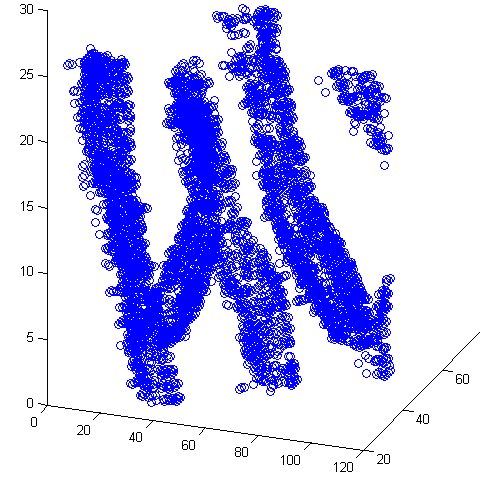
\includegraphics[width=75mm]{paths.png}}
        \caption{\label{Figure 1:} Data extracted from a video of multiple moving targets. The vertical axis denotes the frame number and the two horizontal axes denote $x$ and $y$ coordinate positions, respectively, within a given frame. The data comes from a 50 frame video segment showing 5 moving ants (note that one ant enters the scene near the middle of the segment). The data extraction procedure was set to collect a high density of pixel locations to allow for easier viewing.}
\end{figure}\\
\\
The main goal of the data extraction procedure is to stay simple enough to be applicable to a wide range of videos containing multiple moving targets without the need for a modified procedure when a new setting, filming condition, or collection of targets is encountered. To this ends, this procedure was used without modification for all videos in this study.

The first experiment was performed on a video segment containing two ants moving across a heterogeneous background with many visible features. A frame from this video segment is shown in Figure 2 (a.). The second experiment was performed on a video segment containing five ants, also moving across a heterogeneous background with many visible features. However, relative to the first experiment, the ant-size to frame-size ratio was larger, the ants were travelling at greater speeds, the ants were closer together (a few of the ants briefly come into contact with each other during this video segment), and the background color and texture were more similar to the color and texture of the ant targets. A frame from this video segment is shown in Figure 2 (b.).
\begin{figure}
\centering
{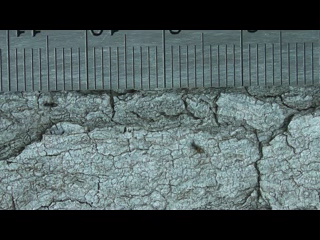
\includegraphics[width=65mm]{antpic1.png}}
\hspace{8mm}
{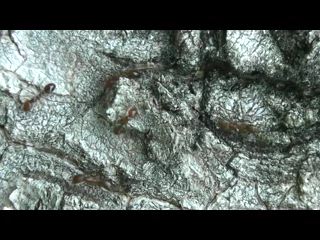
\includegraphics[width=65mm]{antpic2.png}}
\caption{(a.) A frame from the video segment used in experiment one. There are two ants in this image; one is center left and one is center slightly-right.  (b.) A frame from the video segment used in experiment two. There are five ants in this image; four are in a rough diamond shape surrounding the ant in the center.}
\label{test}
\end{figure}

All values in the state of the MCMC sampler needed to be initialized for inference to be be carried out. To start, the number of initial clusters was chosen randomly. To initialize a given cluster's parameters and auxiliary variables at each time step (both of which are used in the inference procedure), an observation was randomly chosen as a seed. The cluster's parameters were then sampled from their posterior distribution given the observation. Using these parameters, the auxiliary variables at an adjacent time step could be sampled from their posterior distribution (as before, making use of the M-H algorithm), which allowed the cluster parameters at the next time step to be sampled. This sampling chain was extended forwards and backwards from the time of the initial observation, allowing the cluster parameters and auxiliary variables to be sampled at all time steps. In this process, the means of the univariate normal distribution followed a random walk of sorts as they were successively sampled. Afterwards, for each observation, the associated assignment variable was randomly assigned to an existing cluster, and the associated deletion variable was drawn from its prior distribution (which entailed drawing a value representing the lifetime of the observation from a geometric distribution, and adding this value to the current time). To illustrate this initialization process, the extracted data from experiments one and two are displyed in Figure 3 (a.) and (b.) below; the shape of each data point represents its associated cluster assignment, and the lines running through the data points represent the paths followed by the mean-component of the cluster parameters during the initial sampling random walk.
\begin{figure}
\centering
{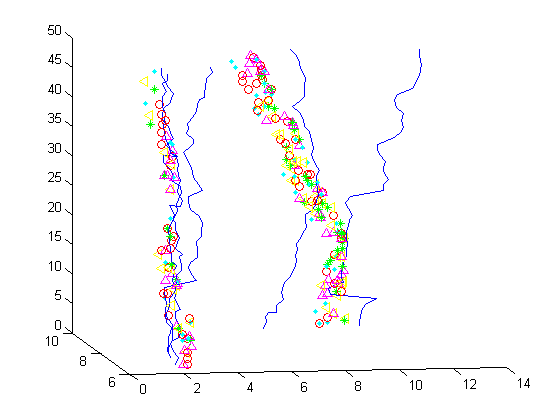
\includegraphics[width=110mm]{exp1_init_3.png}}
\hspace{8mm}
{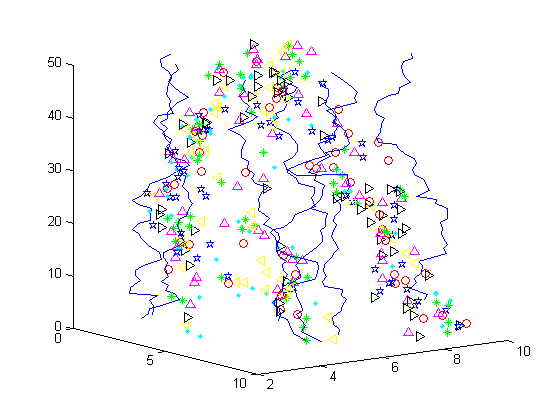
\includegraphics[width=110mm]{exp2_init_5.png}}
\caption{(a.) Initialization of the state in the first experiment. (b.) Initialization of the state in the second experiment.}
\label{test}
\end{figure}




\section{Results}
Results from experiments one and two are shown in Figure 4 (a.) and (b.), respectively. In both cases, the data point assignments seem to predominantly agree, visually, with their membership to their respective worm-like data clouds. Experiment one seemed to separate the worm-like clusters better than experiment two; this is not surprising, as experiment one tracked a much less complex and better separated configuration of targets.
\begin{figure}
\centering
{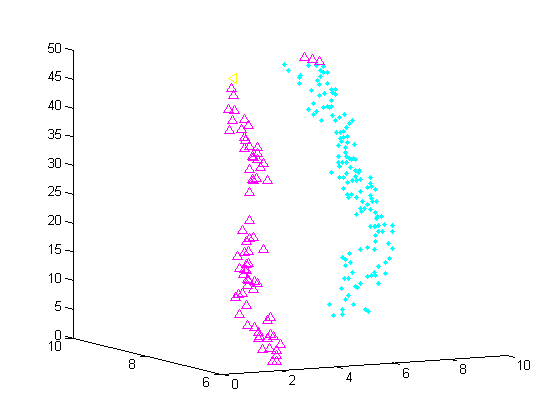
\includegraphics[width=110mm]{exp1_c.png}}
\hspace{8mm}
{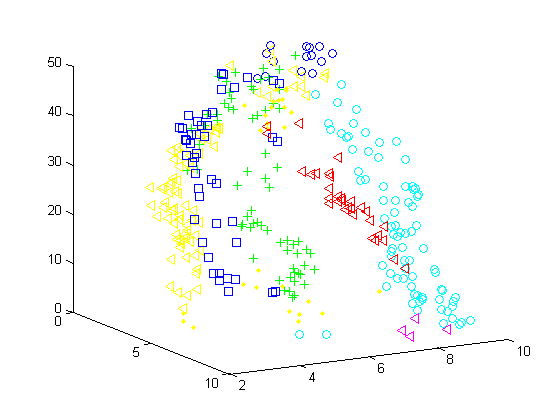
\includegraphics[width=110mm]{exp2_a.png}}
\caption{(a.) Clustering results from experiment one. (b.) Clustering results from experiment two.}
\label{test}
\end{figure}
%
%
%
\\\\ To complete the multiple target tracking process, linear regression was carried out on the data in each isolated cluster. Each regression line was considered the centroid path of a target, and the $\{ x, y \}$ position at which the (vertically oriented) regression line intersected with the horizontal plane of a frame number was considered the target's position at that frame. To account for a small number of false positive assignments, regression was only performed on clusters whose sizes exceeded a specified threshold. The results of regression are shown in Figure 5 (a.) and (b.); a red regression line is overlayed on the plots resulting from the inference procedure.
\begin{figure}
\centering
{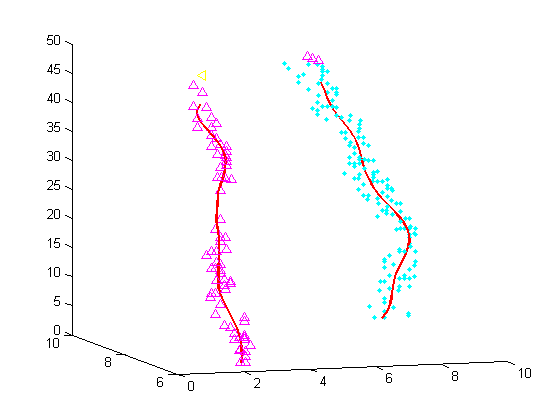
\includegraphics[width=110mm]{exp1_regression.png}}
\hspace{8mm}
{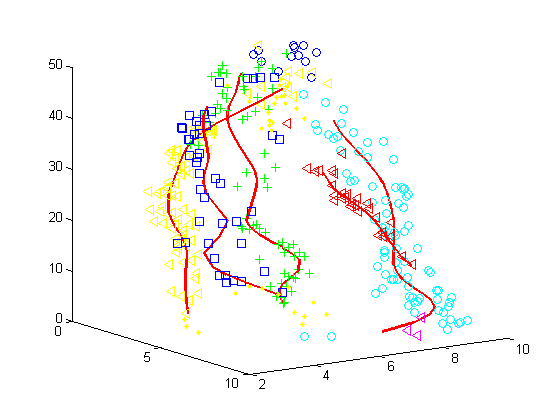
\includegraphics[width=110mm]{exp2_regression.png}}
\caption{(a.) Experiment one results with regression lines. (b.) Experiment two results with regression lines.}
\label{test}
\end{figure}






\section{Conclusion}
This paper has exhibited successful MTT over short video sequences with the use of a time dependent GPUDPM model. The technique was illustrated on two multiple target tracking scenarios involving disparate targets and backgrounds. A general data extraction algorithm was outlined as a simple way to collect data from a wide variety of videos containing multiple moving targets. We hope that this research might help in development of more general MTT algorithms, with the ability to track a large variety of targets with arbitrary characteristics moving over diverse backgrounds 






\begin{small}
\bibliographystyle{plainnat}
\bibliography{refs2} 
\end{small}


\end{document}
